\chapter{Evaluation}
\label{chapt|evaluation}

The evaluation of our work is split in two main sections: first, a formal
feature comparison with other knowledge representation systems (as presented at
section~\ref{sect|surveyed-systems}), then a detailed presentation of several
experimental evaluations that have been conducted during the thesis preparation.

\fxwarning{Do not forget to actually *evaluate* the experiments!}

This two evaluation facets will naturally lead to the conclusion at the next
chapter, where we will draw scientific and technical perspectives that take
into account strengths and weaknesses of our contribution.

%%%%%%%%%%%%%%%%%
\section{Limits of {\tt oro-server}}
\label{sect|limits-oroserver}

\subsection{The left-overs: What ORO does not provide?}

\subsubsection{Representation of time}

In the ORO server, knowledge is mostly atemporal: the set of triples stored in
the server represents the beliefs of the robot \emph{at the current time}. The
robot represents knowledge about the \emph{here and now}.

One exception previously mentioned: when a statement is attached to a memory
profile that is not permanent, the statement is reified and the creation
timestamp is attached to the statement, thus enabling removal after a period of
time that depends on the memory profile.

Statement reification to store timestamps of creation for all statements is
technically very easy to do in ORO server, but has not been actually enabled
because the performance hit (each reified statement produces four triples
instead of one) was not justified by any current use case of ORO server.

\subsubsection{Representation of uncertainty and likelihood}

The challenge of representing and reasoning under uncertainty has not been
tackled in ORO server, at least not \emph{within} the current ORO server
knowledge model. Two reasons explain this absence: the decisional architecture
developed at LAAS for the robots has not consistent approach to uncertainty
representation and management, neither at the \emph{symbol production} level
(\ie SPARK, section~\ref{sect|spark} or {\sc Dialogs},
section~\ref{sect|dialogs}) or at the symbol comsumption level (execution
control). Thus, no strong incentive pushed us in this direction. Then, the
current tools available from the Semantic Web domain to manipulate and reason
about knowledge do not provide mature support for uncertainty management. Some
effort do exist (like the {\sc Pronto} reasoner~\cite{Klinov2008}), but this
does not appear to be a major focus in the currently available tools.


\subsubsection{(Non) Monotonic Reasoning}
\subsubsection{Presupposition accommodation}

\subsubsection{Physics-based reasoning}
\subsubsection{Planning}
Making decision based on prediction

\subsubsection{Advanced Memory Models}

\fxwarning{reinforcement, classification not only on the temporality, but also on the semantic content}

\subsubsection{Justification and Resolution of Cognitive Conflicts}

Logical inconsistencies in one ORO's model (or, from a cognitive point of view,
cognitive conflicts) could be better dealt with: while (partially) provided by
the Pellet reasoner, and output to the developers for debugging purposes, the
logical justification of the inconsistency is not really exploited.



\subsubsection{Relaxation time}

The relaxation time (section~\ref{sect|performances} of ORO for the average
workloads we have encountered during the experiments is in the range of 100ms.
The temporal resolution that follows for the symbolic layer, while acceptable
in most cases, is not satisfactory. In particular, multi-modal interaction
requires fine grained temporal alignement between modalities~\cite{Li2012}
which are not possible with the current temporal performances of ORO.

%%%%%%%%%%%%%%%%%%%%%%%%%%%%%%%%%%%%%%%%%%%%%%%%%%%%%%%%%%%%%%%%%%%%%%%%%%%%%%

\section{Comparison of {\tt oro-server} with other existing systems}
\label{sect|evaluation-oroserver}

This section tries to summary the various approaches we surveyed in the
previous sections and to draw some research perspectives. This section does not
exactly follow the list of compared features presented in
section~\ref{sect|features}. We have organized it along four axis: \emph{what
can be represented?}, \emph{How knowledge is created and grounded?}, \emph{What
can be done with the knowledge?} and \emph{How to use knowledge in the whole,
larger robot architecture?}.

Table~\ref{table|contribution-by-systems} proposes a summary of the main scopes
of \emph{contribution} of the systems we have surveyed. This overview helps to
identify the main weaknesses of current approaches of knowledge representation
regarding the long-term goal of \emph{human-level robots}.

\begin{landscape}
\begin{table}\tiny
\begin{center}
\begin{tabular}{p{0.2cm}p{3.4cm}p{1.6cm}p{1.3cm}p{1.5cm}p{1.7cm}p{1.5cm}p{2cm}p{1.4cm}p{1.4cm}p{1.4cm}|p{1.4cm}}
\toprule
\multicolumn{2}{c}{\bf Category}                                                     & ARMAR \cite{Holzapfel2008}& CAST \cite{Hawes2007}       & GLAIR \cite{Shapiro2009}    & GSM \cite{Mavridis2006}     & {\sc Ke Jia} \cite{Chen2010}& {\sc KnowRob} \cite{Tenorth2009a}  & NKRL \cite{Sabri2011}           & OUR-K \cite{Lim2011}          & PEIS \cite{Daoutis2009}       & ORO \cite{Lemaignan2010}                      \\
                                                                                                                                                                                                                                                                                                                                                                                                                                
\midrule                                                                                                                                                                                                                                                                                                                                                                                                                        
                                                                                                                                                                                                                                                                                                                                                                                                                                
\multirow{4}{*}{\turn{90}{\bf Expressiveness}}                   & Logical formalism & TFS                       & (none)                      & SNePS                       & (none)                      & ASP                         & Prolog                             &                                 & DL + Horn clauses             & {\sc CycL}                    & DL (OWL)                                      \\
                                                                           & OWA/CWA &                           &                             &                             &                             & CWA                         & CWA                                &                                 &                               &                               & OWA                                           \\
                                                              & Modeling uncertainty &                           &                             &                             & ++ (stochastic models)      &                             & {\it+++} \cite{Jain2009}           & +                               & + (\emph{candidate} entities) &                               &                                               \\
                                                                    & Meta-cognition &                           &                             &                             &                             &                             & ++                                 &                                 &                               &                               & ++ (reification, taxonomy walking)            \\
\hline                                                                                                                                                                                                                                                                                                                                                                                                                          
\multirow{7}{*}{\turn{90}{\bf Representation}}                & Space Representation &                           &                             &                             &                             &                             &                                    &                                 & ++                            &                               &                                               \\
                                                               & Time representation &                           &                             &                             & ++ (snapshots)              &                             &                                    &                                 & +                             &                               &                                               \\
                                                                    & Actions/Events &                           &                             &                             & ++ (events classifiers)     &                             &                                    &                                 & +++                           &                               &                                               \\
                                                                           & Context &                           &                             &                             &                             &                             &                                    &                                 & ++                            & ++ (microtheories)            &                                               \\
                                                                          & Modality &                           &                             &                             & ++ (recursive model)        &                             &                                    & ++                              &                               &                               & +++                                           \\
                                                                     & Introspection &                           &                             &                             &                             &                             & + (SRDF) \cite{Kunze2011}          &                                 &                               &                               &                                               \\
                                                                     & Memory models &                           &                             &                             &                             &                             &                                    &                                 &                               & +                             & +                                             \\
\hline                                                                                                                                                                                                                                                                                                                                                                                                                          
\multirow{9}{*}{\turn{90}{\bf Reasoning}}                   & Standard FOL reasoning &                           &                             &                             &                             & +++                         & +++                                &                                 & +                             & ++                            & ++                                            \\
                                            & Instantiation and structure alteration & ++                        &                             &                             &                             & ++                          & + (dynamic instantiation)          &                                 &                               &                               & ++ (TBox alteration)                          \\
                                                                   & Lazy evaluation &                           &                             &                             &                             &                             & +++ (Prolog, \emph{computables})   &                                 &                               &                               &                                               \\
                                                           & Non-monotonic reasoning &                           &                             &                             &                             & +++ \cite{Ji2011}           &                                    &                                 &                               &                               &                                               \\
                                                      & Presupposition accommodation &                           &                             &                             & +++                         &                             &                                    &                                 &                               &                               &                                               \\
                                    & Prediction, projection, diagnosis, explanation &                           &                             &                             &                             &                             &                                    &                                 &                               &                               & + (explanation)                               \\
                                                                     & Task planning &                           &                             &                             &                             & ++ \cite{Ji2011}            & +                                  &                                 & +                             & {\it++}                       & {\it+++}                                      \\
                                                           & Physics-based reasoning &                           &                             &                             &                             & +                           & {\it+++} \cite{Kunze2011a}         &                                 &                               &                               &                                               \\
                                                                          & Learning & ++                        & ++ \cite{Jacobsson2008}     &                             &                             &                             &                                    &                                 &                               &                               &                                               \\
\hline                                                                                                                                                                                                                                                                                                                                                                                                                          
\multirow{5}{*}{\turn{90}{\bf Acquisition}}                         & Cross-modality &                           & ++                          &                             & +++ (amodal model)          &                             &                                    &                                 &                               & ++ (ambient intelligence)     & {\it+++}                                      \\
                                                                               & NLP & +++                       & +++ \cite{Kruijff2010a}     &                             & +++                         & +++                         &                                    &                                 &                               & + (template-based)            & {\it+++} \cite{Lemaignan2011a}                \\
                                                                     & Web Resources &                           &                             &                             &                             &                             & {\it+++} \cite{Nyga2009}           &                                 &                               &                               &                                               \\
                                                                         & Grounding &                           & ++                          &                             & ++ (bidirectional)          &                             & +++ (semantic maps) \cite{Blodow2011} &                              & +++ (bottom-up)               & +++ \cite{Loutfi2008}         & {\it++} (amodal model) \cite{Lemaignan2012}   \\
                                                              & Intrinsic Motivation &                           & ++ \cite{Hawes2011}         &                             &                             &                             &                                    &                                 &                               &                               &                                               \\
\hline                                                                                                                                                                                                                                                                                                                                                                                                                          
\multirow{4}{*}{\turn{90}{\bf Integration}}     &   \ldots with sensori-motor layers &                           &                             &                             & +                           &                             & +++ (\emph{computables})           &                                 & +                             & ++ (\emph{tuple space})       &                                               \\
                                                      & \ldots with executive layers &                           & ++ (ubiquitous events)      &                             & +                           &                             & ++ (language extensions) \cite{Beetz2010} &                          & ++                            & ++ (\emph{tuple space})       & ++ (\emph{semantic events})                   \\
                                                          & Monitoring and debugging &                           &                             &                             &                             &                             &                                    &                                 &                               &                               & {\it+} (remote visualisation)                 \\
                                                           & Performances evaluation &                           & ++ \cite{Hawes2008}         &                             & ++ (Token test)             & +                           & + \cite{Tenorth2011}               &                                 &                               &                               &                                               \\

\bottomrule

%\end{tabularx}
\end{tabular}
\end{center}

\caption{Main domains of contribution of current KRS. Italics mean that the
feature is implemented as an external module. Main references are given in the
table header. When relevant, feature-specific publications have been provided.
An empty cell means that either the system does not contribute to this domain
or we could not find relevant literature.}

\label{table|contribution-by-systems}
\end{table}
\end{landscape}

%%%%%%%%%% Underlying knowledge model table %%%%%%%%
\begin{table}
\begin{center}

\begin{tabular}{ll}
\toprule
{\bf Project} & {\bf Common-sense knowledge source} \\
\midrule
ARMAR/{\sc Tapas} & Custom ontology related to the kitchen\\
CAST Proxies &  None \\
GLAIR & None\fxwarning{Check that!} \\
GSM &  Predefined categories \\
Ke Jia & None \\
{\sc KnowRob} & {\sc OpenCyc}, processed web content, custom OWL-DL ontology \\
NKLR &  None \\
OUR-K & {\it A priori} knowledge structure and axioms, custom set of instances\\
ORO & {\sc OpenCyc}, custom OWL-DL ontology \\
PEIS Ecology & {\sc ResearchCyc} \\

\bottomrule

\end{tabular}
\end{center}
\caption{Underlying knowledge sources for each project}
\label{table|knowledge-sources}
\end{table}


\subsection{Performances Analysis}

\fxwarning{Mention reasoning and expresiveness, cf section oro-server}

\section{Experimental evaluation}
\label{sect|experimental-evaluation}

Experimental validation of our work takes several forms that are presented in
this section.

First, it must be noted that our experiments are largely independant from the
underlying platform. Since our contributions are mainly at the symbolic
reasoning level, we rely on intermediate layers for the back and forth
conversion of sensori-motor data to symbols. These intermediate layers are
obviously much more dependant on the platform.

We present here three distinct experimental frameworks: first, we present the
MORSE simulator (section~\ref{sect|simulation}) that has been developed during
the thesis preparation with several features dedicated to human-robot
interaction simulation.

Then, several more ``traditional'' experiments on different robotic platforms
are presented (sections~\ref{sect|casestudies}, \ref{sect|expe1}
and~\ref{sect|expe2}). Most of these experiments have been conducted at
LAAS-CNRS and in other laboratories involved in the European CHRIS project
(\emph{Jido}, \emph{PR2}, \emph{ICub} and \emph{Bert} platforms).  Experiments
have also been conducted at Munich's IAS laboratory on the \emph{Rosie}
platform.

Finally, we report in section~\ref{sect|roboscopie} on the theater performance
\emph{Roboscopie} that was presented in 2011 at a large general public audience
in Toulouse.

\subsection{Simulation of HRI interaction}
\label{sect|simulation}

\subsubsection{The MORSE simulator}

The Modular OpenRobots Simulation Engine (MORSE)~\cite{Echeverria2011}
(figure~\ref{fig|morse-gui}) is a open-source tool developed for robotics
research. It is a domain independent simulator, where virtual robots can
interact with a 3D environment, using sensors and actuators that behave in the
same way as their counterparts in the real world.  MORSE relies on the advanced
3D (OpenGL shaders) and physics simulation ({\sc Bullet} physics engine)
capabilities of the Blender \emph{Game Engine}, a real-time 3D runtime
integrated to the open-source Blender modeling toolkit.  This allows for
semi-realistic simulation of complex environments.

\begin{figure}[t]
      \centering
      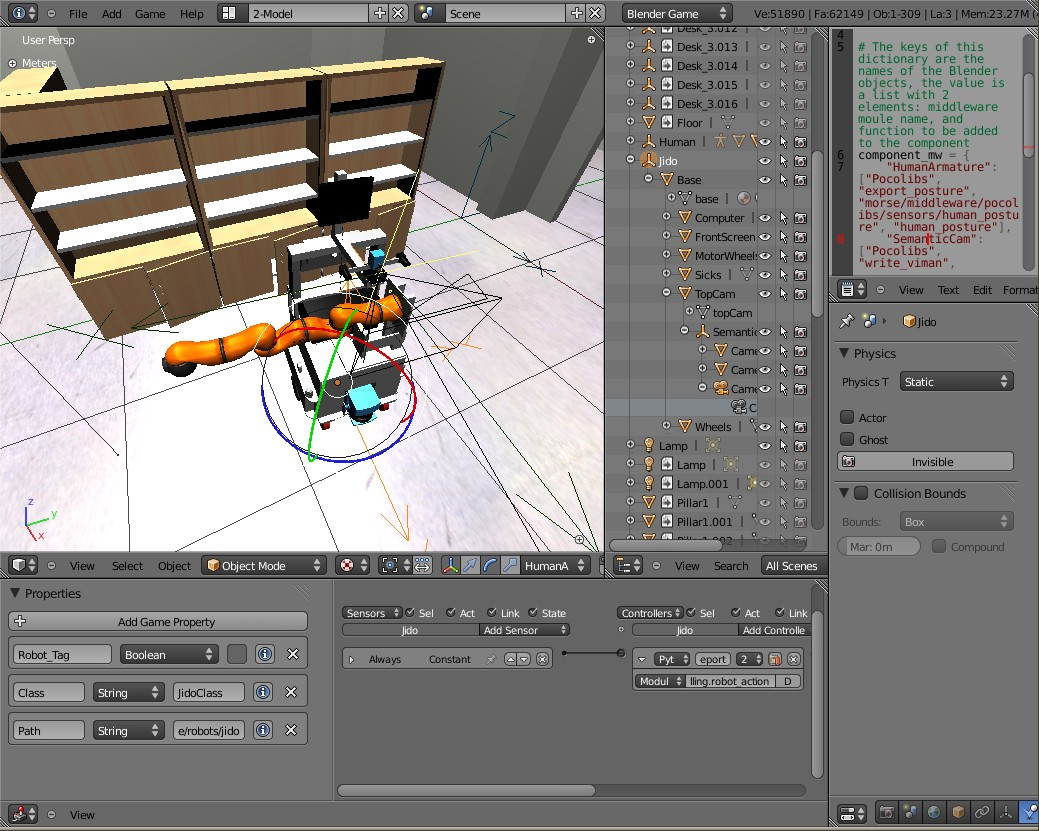
\includegraphics[width=0.7\columnwidth]{experiments/morse-interface.jpg}
      \caption{Screenshot of the MORSE graphical interface (inside Blender).}
      \label{fig|morse-gui}
\end{figure}


The MORSE components (sensors and actuators) exchange data with the robotics
software via middleware bindings, using a \emph{Software In The Loop} (SAIL)
architecture. Middleware supported in the current version include LAAS'
Pocolibs library, ROS and YARP, as well as a socket-based raw protocol. This
design allows in principle to use the same software in both the real robots and
the simulator. Instructions given to the robot are interpreted in the simulator
to provide the control of actuators, such as the motion of the robot and its
arms.  The data from simulated sensors is sent back through the middlewares,
{\it e.g.}~exporting the images from cameras, or the positions of the robot,
human and other objects of interest.

MORSE provides support for several classes of robots \textit{out of the box}, and
allows for easy customization of those, either by composing individual sensors
and actuators with empty robot structures directly in the MORSE interface, or
through a Python-based script language that permits to conveniently describe
robots and simulation scenarii.

Other experiments using simulation have been carried to gather data for HRI
\cite{Chernova2011}. However, these do not involve the actual robot software,
and it is another human who takes the role of the robot.

\paragraph{Contribution} While not directly linked to the main topic of this
thesis, I have been deeply involved in the design and development of MORSE: I'm
responsible for most of the original software design, and large parts of the
core foundations of the project.

\subsubsection{HRI specific features}
\label{sect|morse-hri}

\begin{figure}[t]
      \centering
      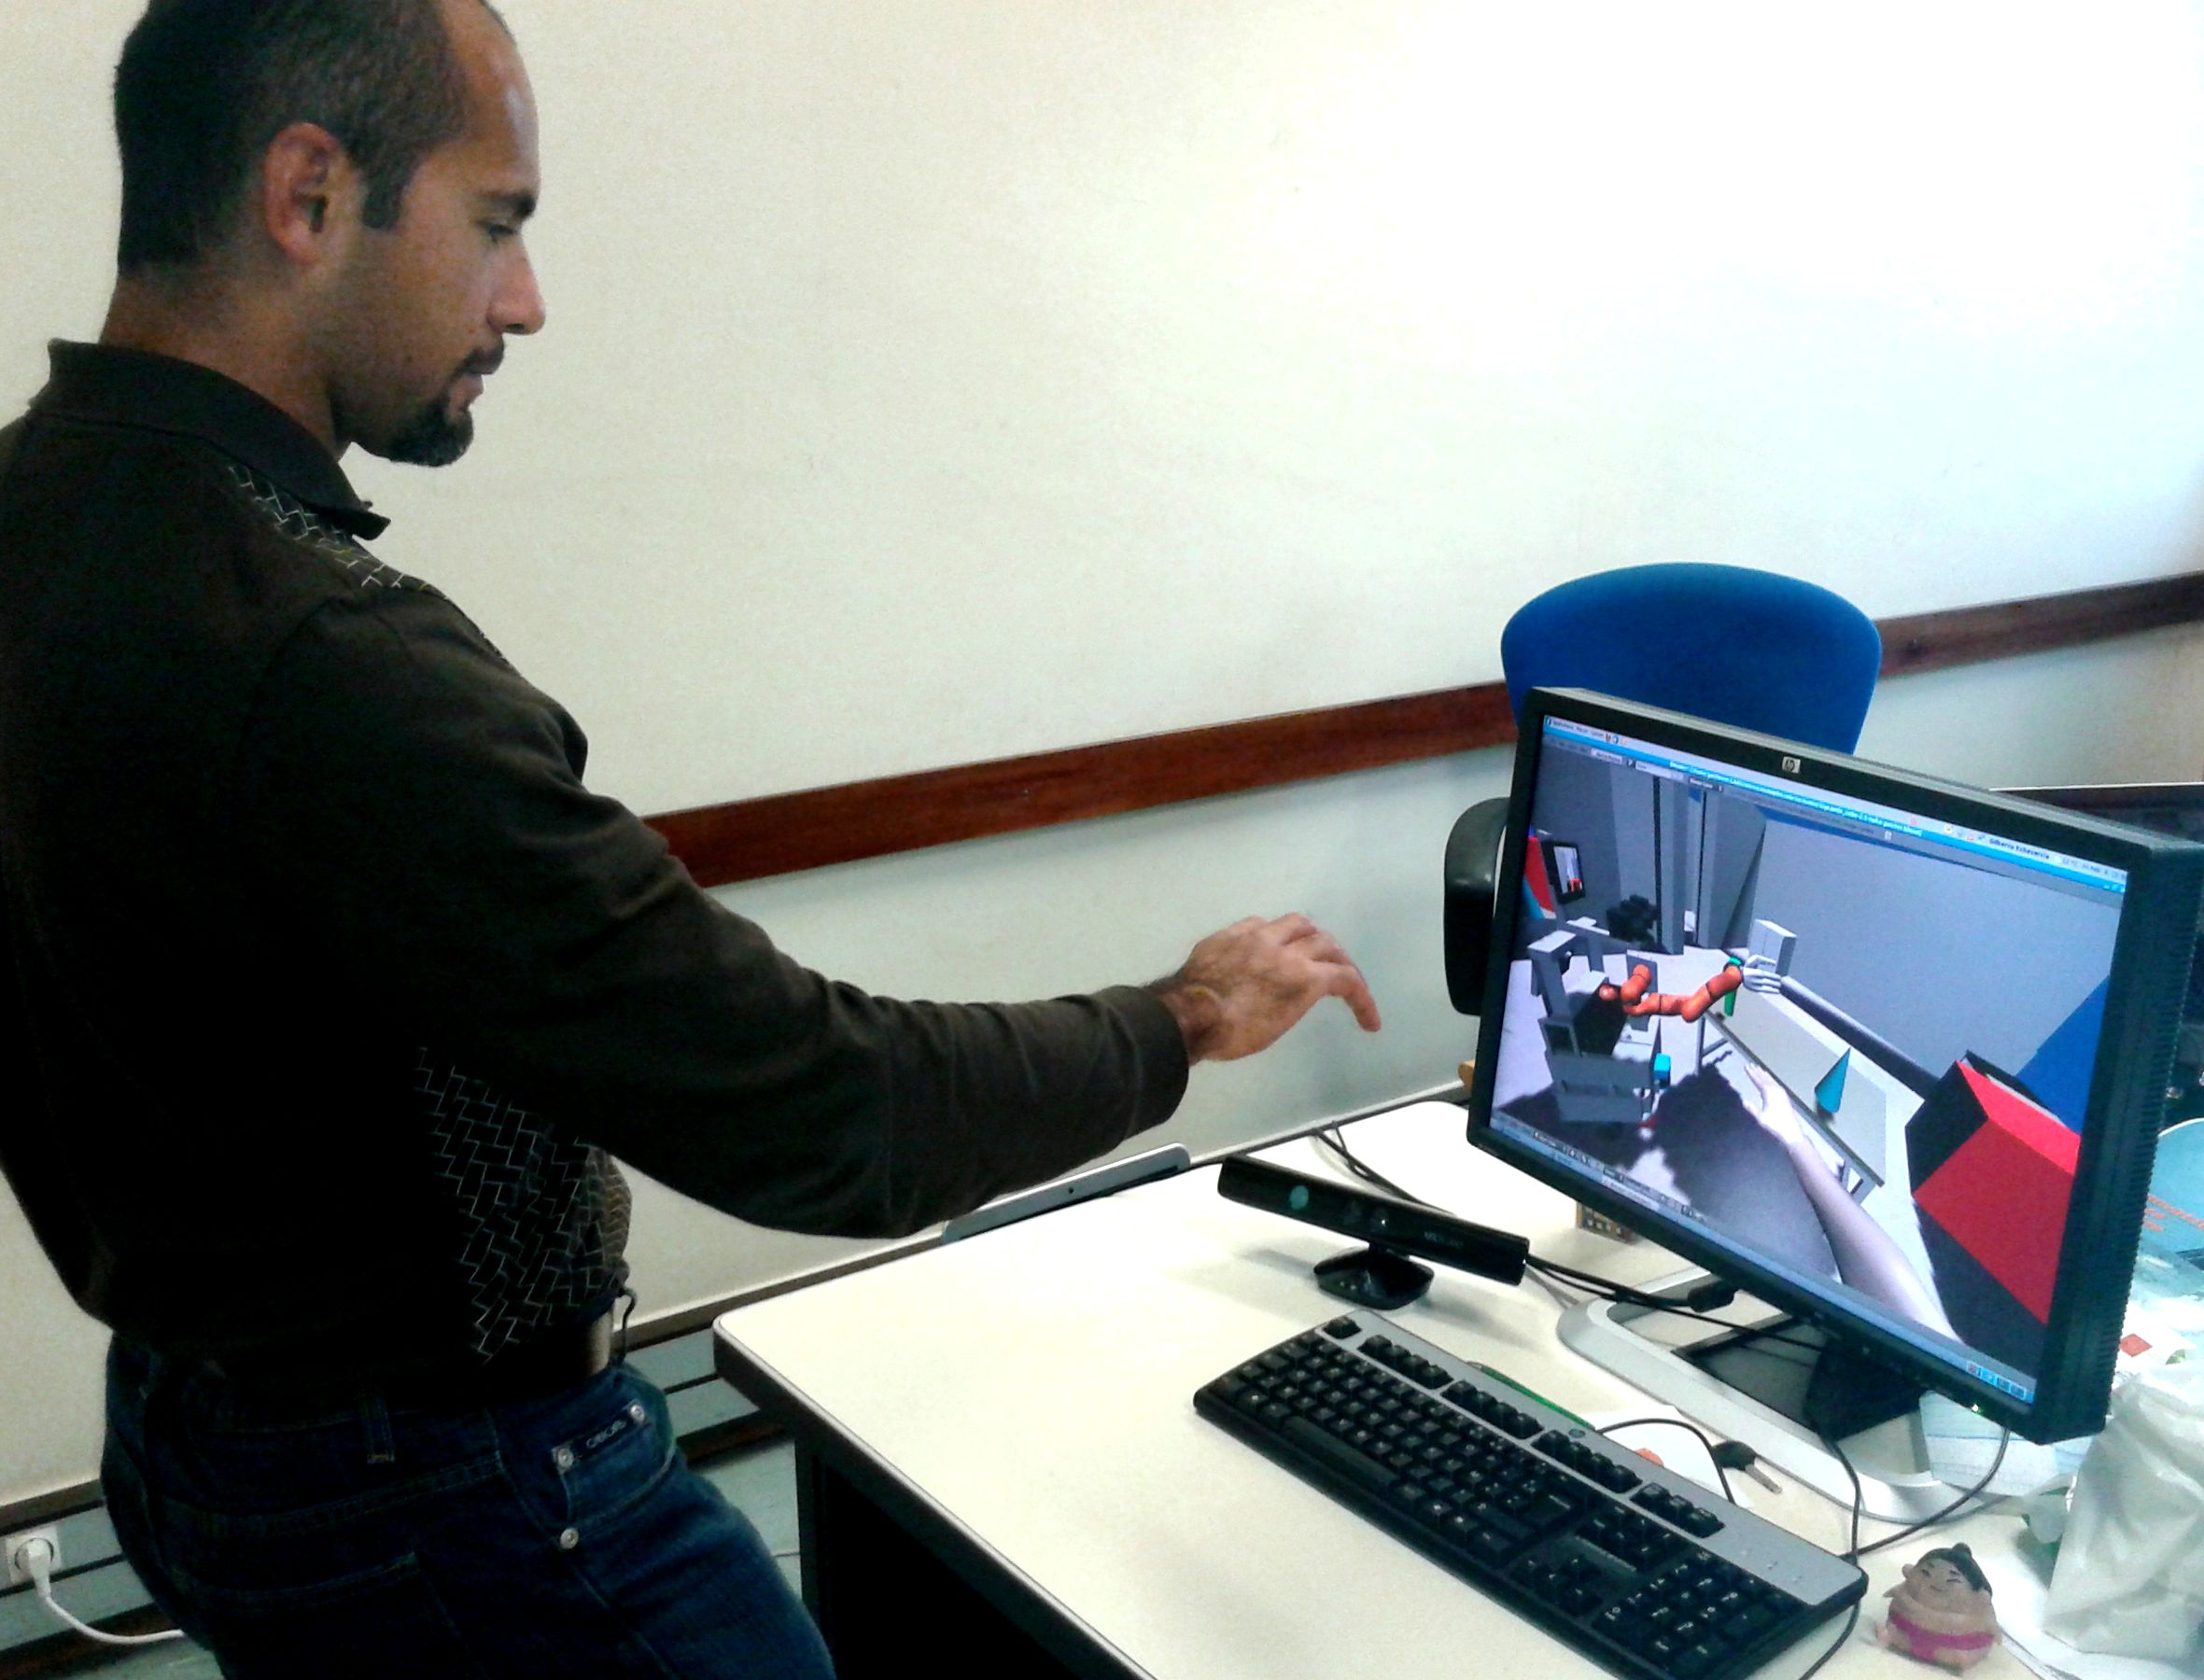
\includegraphics[width=0.7\columnwidth]{experiments/morse-kinect.jpg}
      \caption{The experimental setup with the human avatar controlled from a
      Kinect.}
      \label{fig|kinect-setup}
\end{figure}

An interactive \emph{human avatar} is available in MORSE. It provides a
first-person immersive experience: when started, one can take the role of the
human and control it via the keyboard, a WiiMote or through a Kinect device
(Fig.~\ref{fig|kinect-setup}).

When in first-person mode, the user can interact in several ways with the
environment. He/she can pick and release objects, can open drawers and
cupboards. As any other object, the avatar physically interacts (collision
detection) with the surrounding furnitures.  MORSE exports the position
and posture of the avatar as a global joint state to be used by the real
software components of the robot.

MORSE also offers a special sensor that exports abstracted informations of
objects visible to the robot (called the \emph{semantic camera}). This
sensor typically exports the name, type (glass, table, bottle, etc.), color and
location of objects. Since human-robot interaction often involves
semantic-rich environments, this abstract sensor simplifies the
experiments on such scenarii, by avoiding the added complexity of processing
camera images to detect the objects of interest and exploiting the inherent
knowledge of the simulated world.

\subsubsection{An Experimental Framework}

Due to its nature, MORSE offers two main advantages compared to experiments on
a real robot: light-weight deployment and repeatability. MORSE is already used
for human-robot interaction both at the LAAS-CNRS and at the Technical
University of Munich, Germany.

MORSE is integrated to the LAAS architecture.  In particular, both the human
posture and the object features are integrated with SPARK, a
module dedicated to geometric and temporal reasoning.  This module is a key
component providing a base of facts such as objects' relative placements,
visibility and reachability by the agents present in the scene. It additionally
provides a stable state of the world to the motion planners.

\subsection{Case Studies}
\label{sect|casestudies}

This section reports on three small experiments conducted in the first half of
the PhD thesis preparation. Each of them illustrate one specific aspect of the
knowledge base.

The first experiment, \emph{Point \& Learn} shows how the structure
(\emph{TBox}) of the knowledge base can be altered (in this case expanded) at
runtime through pointing interaction.

The second experiment, \emph{Odd One Out} shows how the knowledge model can be
used along with the categorization routines to isolate an ``odd" object, given
a simple context.

Lastly, the third case study is an implementation of the \emph{Spy Game} where
one of the player think of an object and the other one must guess by asking
questions.

It must be noted that these three experiments have been implemented on three
distinct robotic platforms: the \textit{BERT2} robot from the Bristol Robotics
Laboratory (a YARP-based architecture), the \textit{Rosie} robot from the
Technical University of Munich (a ROS-based architecture) and the \textit{Jido}
robot at LAAS-CNRS (based on the LAAS Pocolibs middleware).

\subsubsection{Knowledge Acquisition: Point \& Learn}
\label{expe|pointandlearn}

\begin{figure}
\centering

\centering
  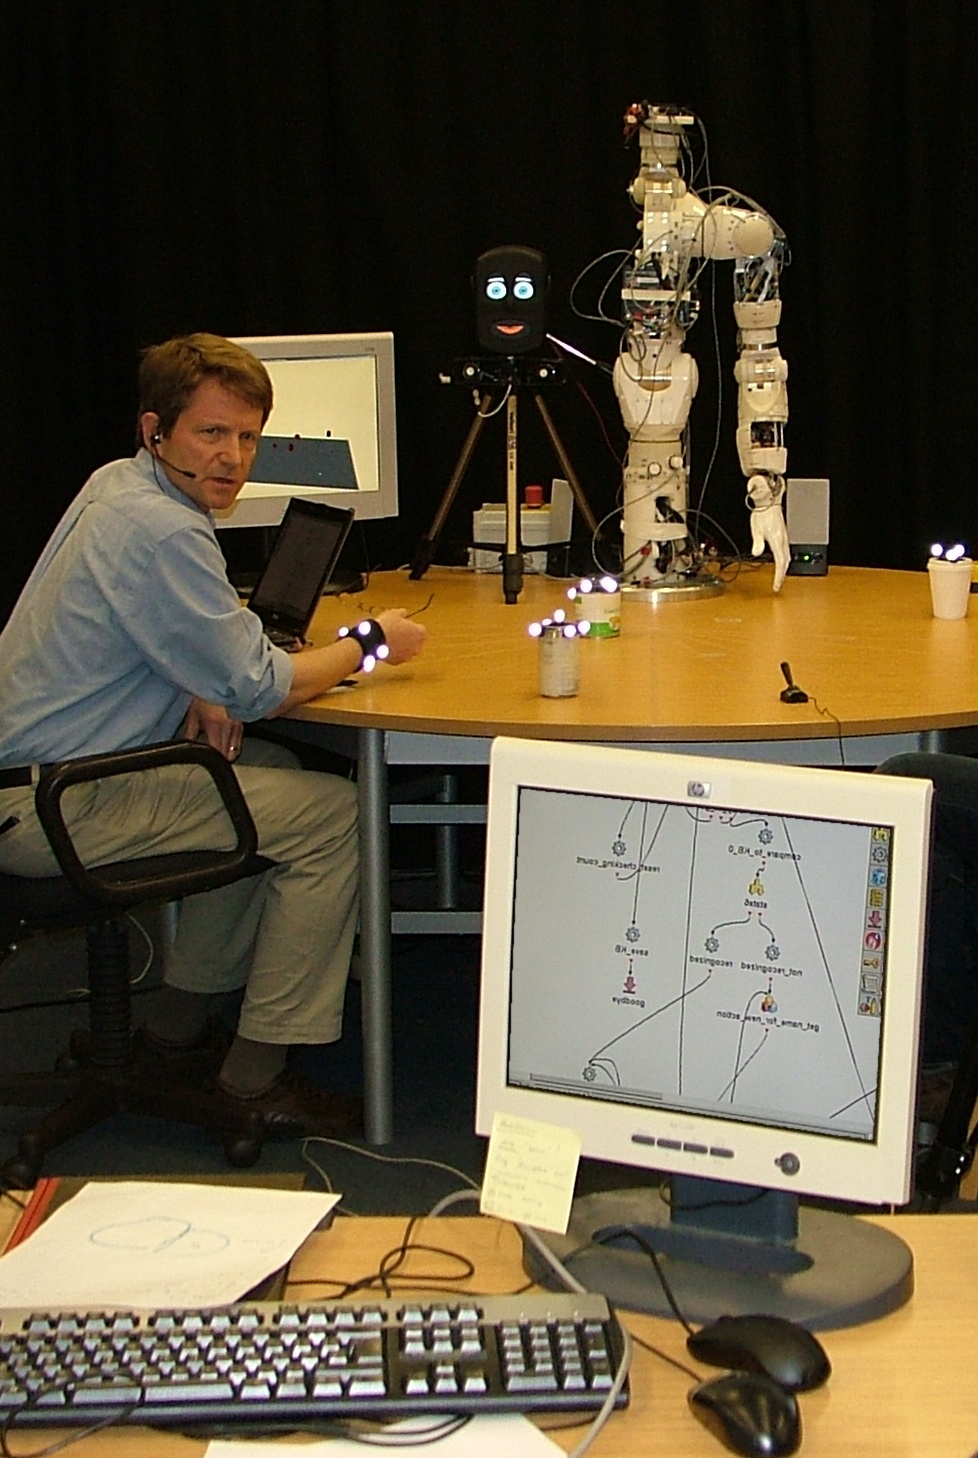
\includegraphics[width=0.4\columnwidth]{experiments/bristol_integration.jpg}
  \caption{Teaching the Bert robot new objects}
  \label{fig|bristol}

\end{figure}

We have implemented a \textit{Point \& learn} behaviour on the Bert
robot~\cite{Lallee2010b} (Figure~\ref{fig|bristol}): the user shows an object
to the robot, and if the robot sees it for the first time, it will ask for its
name and type.

The object perception module relies on motion capture (VICON system) to
identify and localize objects. A so-called \textit{primitive detection} module
is responsible for updating ORO with the list of objects currently seen by the
robot as well as their state (moving or not) and their relations to other
objects (touching or not). On the other end, a human-robot interface based on
the CLSU Toolkit\footnote{\url{http://cslu.cse.ogi.edu/toolkit/}} is in charge
of speech recognition, speech synthesis and basic natural language processing.

By querying ORO for moving objects, the interface retrieves the object ID that
has the focus of attention (last moving object), and asks the human for a name
and a type if the object is new. Figure~\ref{tab|transcript_bert} reproduces a
typical dialog with Bert.

At the end of this sequence, two more RDF statements are added to the robot
knowledge base: \texttt{[5001 rdfs:label "coffee-cup"]} and \texttt{[5001
rdf:type Cup]}.

\begin{figure}[!ht]
\centering
	\begin{tabular}{r|p{0.6\columnwidth}}
	\chatN{bert} & Initializing... \textit{[about 5 sec]} ...What's next? \\
	\chatN{human} & \textit{[moves an object]} \\
	\chatN{bert} & \textit{[does not know the object]} How is it called? \\
	\chatN{human} & coffee-cup \\
	\chatN{bert} & Did you say coffee-cup? \\
	\chatN{human} & yes \\
	\chatN{bert} & Ok. Now I know. What kind of object is coffee-cup? \\
	\chatN{human} & a cup \\
	\chatN{bert} & Did you say cup? \\
	\chatN{human} & yes \\
	\chatN{bert} & So coffee cup is a cup. What's next? \\
	\end{tabular}
	\caption{Transcript of a chat with the Bert robot}
	\label{tab|transcript_bert}
\end{figure}

Due to the limitation of the speech recognition software, only a predefined set
of names or types could be recognized, thus preventing the robot to add
completely original objects.

\subsubsection{Odd One Out}
\label{expe|odd_one_out}

\begin{figure}
\centering

    \subfigure[]{
        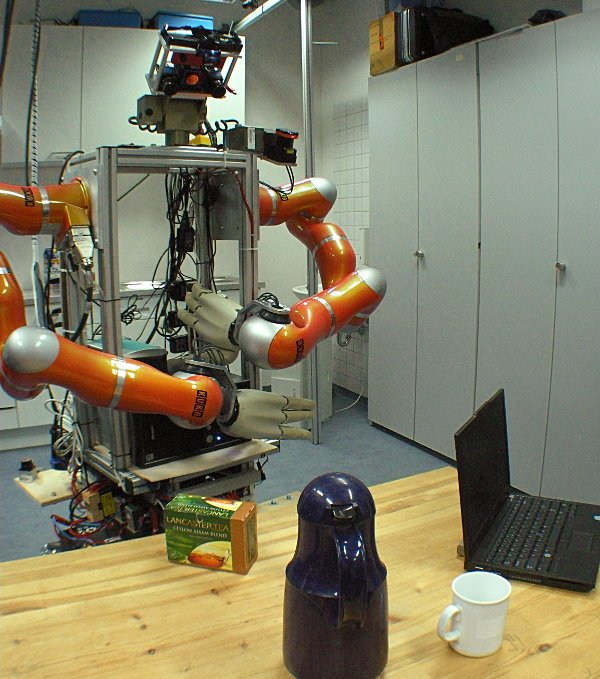
\includegraphics[width=0.4\textwidth]{experiments/kimp1.jpg}
    }
    \subfigure[]{
        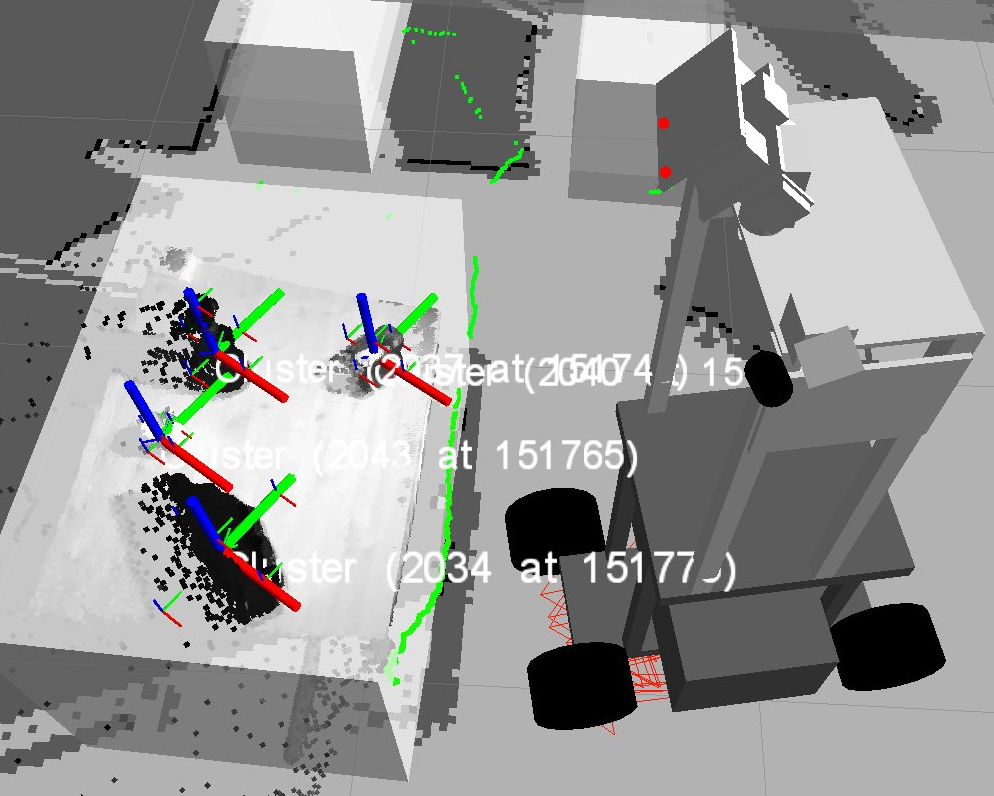
\includegraphics[width=0.4\textwidth]{experiments/rviz.png}
    }

    \caption{(a) Rosie, looking for objects it may know, and (b) viewed in
    RViz. The clusters of point are given an unique identifier by the
    perception that allow the supervision create the link between the physical
    objects and their symbolic representation in ORO.}

\label{fig|kimpwatching}
\end{figure}


The \emph{Odd One Out} scenario extends the \textit{Point \& Learn} experiment
and completes an on-going experiment at the IAS laboratory where a robot is
asked to list missing items on a table being set, based on probabilistic
reasoning on previously recorded observations.
%~\cite{Pangercic2009}.

We use ORO to introduce human interactions and common-sense reasoning: the
robot picks an unknown object from the table, shows it to the user, and asks
about its name and type (Figure~\ref{fig|kimpwatching}). The user continues to
describe the object (through concepts) until a concept known by the robot is
given. The learning process starts over again with another unknown object. Once
all objects are learned, the robot tells which objects do not belong to a
typical breakfast table (\textit{i.e.} objects that are neither food or
tableware). The human interacts with the robot through a dedicated XMPP bridge,
allowing to chat with the robot with a standard Jabber messaging client.
Figure~\ref{tab|transcript_kimp} corresponds to a chat session with Rosie.

The supervision (\textsc{cram}\footnote{\textsc{cram} (Cognitive Robotic
Abstract Machine) is a RPL-derived framework for rapid development of cognitive
robot control programs we currently develop.}~\cite{Beetz2010}) automatically
updates the ORO server whenever an object enters or leaves the field of view
(the perception is based on the \textsc{CoP} framework~\cite{Klank2009}).
Therefore, the integration of ORO can be seen as an extension to the robot's
belief state that not only contains abstract identifiers of the internal object
representation used in plans, but also the semantics and roles of objects in
the scenario.

\begin{figure}[!ht]
\centering
	\begin{tabular}{r|p{0.7\columnwidth}}
	\chatN{rosie} & Servus! The Bavarian robot is up and fit! \\
	\chatN{rosie} & What is the name of the WHITE CLUSTER on the TABLE? \\
	\chatN{human} & "Rosie's mug" \emph{[Rosie adds \stmt{OBJ001 rdfs:label "Rosie's mug"} stmt]}\\
	\chatN{rosie} & What kind of object is Rosie's mug? \\
	\chatN{human} & Mug \\
	\chatN{rosie} & What is a Mug? \emph{[Rosie adds \stmt{OBJ001 rdf:type Mug} but it does not know the \emph{Mug} concept]}\\
	\chatN{human} & Tableware \emph{[Rosie knows about \emph{Tableware} - belongs to the common-sense ontology. It adds \stmt{Mug rdfs:subClassOf Tableware}]}\\
	 & (...) \\
	\chatN{rosie} &  What is the name of the BLACK CLUSTER on the TABLE? \\
	\chatN{human} & my laptop \\
	\chatN{rosie} & What kind of object is my laptop? \\
	\chatN{human} & Computer \\
	\chatN{rosie} & What is a Computer? \\
	\chatN{human} & Artifact \\
	\chatN{rosie} & Do you want me to learn more objects? \\
	\chatN{human} & no \\
	\chatN{rosie} & These objects are odd: my laptop \\
	\end{tabular}

    \caption{Transcript of a Jabber session with the robot Rosie. Compared to
    dialog with Bert (\ref{tab|transcript_bert}), we see here that the robot
    anchors the new objects in its already acquired knowledge.}
	
	\label{tab|transcript_kimp}
\end{figure}

By asking in loop the human for the categories of an object until it can
connect it to a concept it already knows, the robot accurately anchors
perception in its symbolic model and it is able to reason about it. At the end
of the experiment, the robot identifies and returns the odd objects for the
breakfast table (\textit{i.e.}, in our example, objects that are neither
\texttt{Tableware} or \texttt{Food}).

An unexpected example of what the symbolic reasoning layer brings to more
traditional robotic architectures emerged during the \emph{Odd One Out}
experiment: the perception routines provided segmented blobs corresponding to
objects, along with their colours. The supervision would then feed ORO with the
visible objects. At some point, ORO suddenly refused to add an object. What
seemed at first a communication bug between modules, was actually the
consequence of a consistency check by ORO: Because of bad light conditions, the
color recognition was not very reliable, and the same object was set to have
two different colours at the same time. That was inferred as impossible by ORO
and thus discarded. This kind of logical failure can be used to improve
low-level perception results by ``closing the loop'' with high-level, symbolic
knowledge.


\subsubsection{The Spy game}
\label{spygame}

This game is based on the traditional children game ``I Spy''. The idea is to
discover the object or concept one of the participants is thinking of by asking
questions such as: ``Is it green? Is it a machine? Is it on your left?'', etc.
When playing, children exploit their knowledge about the world while
categorizing and describing objects through useful discriminants that allow
them to find out the answer as fast as possible while including perspective
taking abilities~\cite{Moll2006}.

\begin{figure}
\centering

    \subfigure[]{
        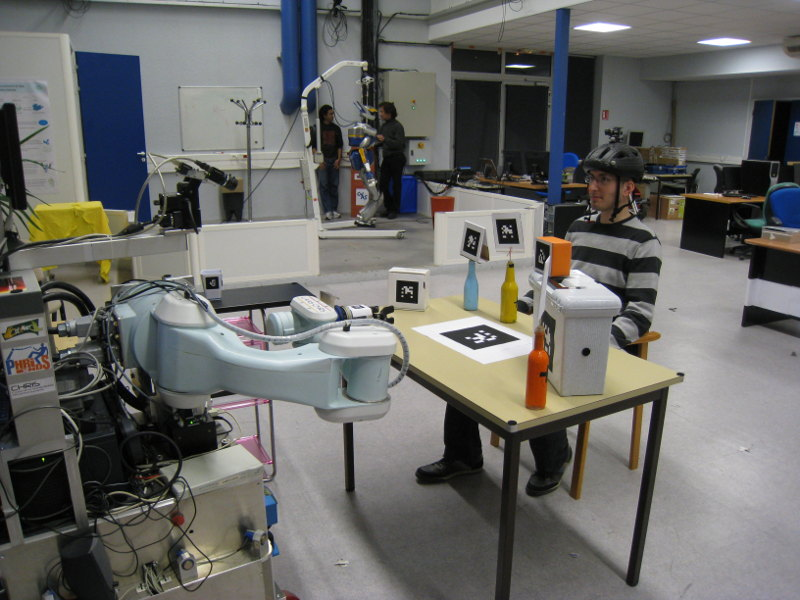
\includegraphics[width=0.4\textwidth]{experiments/spy-game-real.jpg}
    }
    \subfigure[]{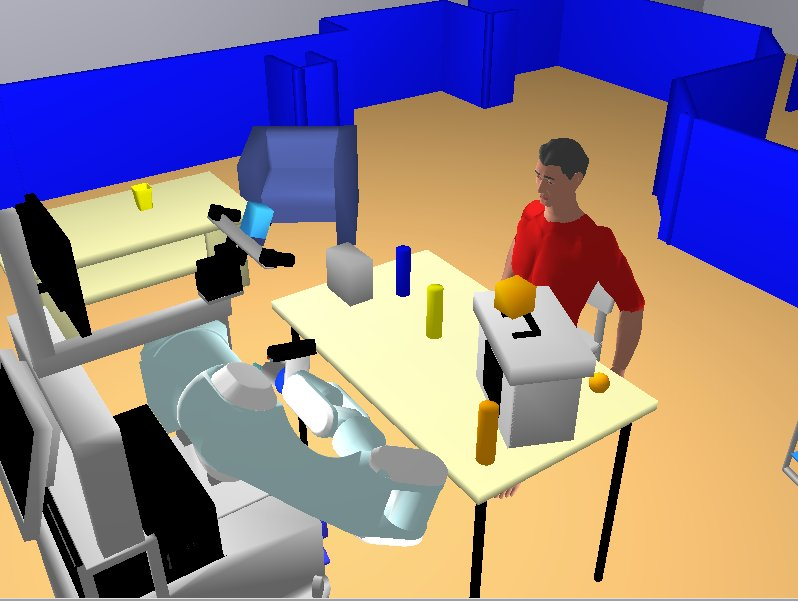
\includegraphics[width=0.4\textwidth]{experiments/spy-game-mhp.jpg}
    }
\caption{Spy game scenario: (a) Real environment and (b) 3D environment model, viewed in \textsc{Move3D}.}
\label{fig|spyGameScenario}
\end{figure}

The scenario for this game (Figure~\ref{fig|spyGameScenario}) consists on a
face-to-face interaction where the human thinks of an object present in the
environment, while the robot queries the human until either discovering the
object or giving up, if no object was found. A categorization example is
presented in Figure~\ref{fig|objectsSpyGame}. The game starts with the human
user giving a first hint (communication is done through a keyboard and screen),
allowing the robot to start the search filtering those objects that fulfill
this first description. Based on this subset, ORO provides a descriptor (or set
of descriptors) that allows a maximum discrimination among objects in the
subset. The robot queries the user about the value of the descriptor (or the
most discriminant among the set of descriptors) and with this new information,
the current subset of objects is filtered again. The process is repeated until
either obtaining a single object that fulfills all the descriptor values, or
failing (\textit{i.e.} no object found). 

\begin{figure}[!h]
\centering
\begin{scriptsize}
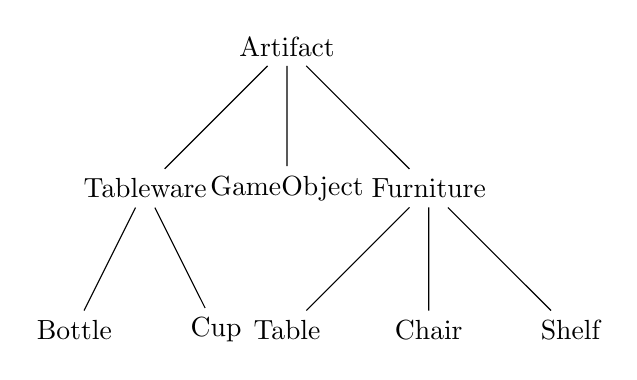
\begin{tikzpicture}[scale=1.2] %[level/.style={sibling distance=30mm/#1},scale=0.8]
	%[edge from parent fork down,
	%every node/.style={fill=black!30,rounded corners},
	%[parent anchor=east,child anchor=west,grow=east,
	%edge from parent/.style={thick,draw}]
	\node {Artifact}
	child {node {Tableware}
		child {node {Bottle}}
		child {node {Cup}}
		}
	child {node {GameObject}}
	child {node {Furniture}
			child {node {Table}}
			child {node {Chair}}
			child {node {Shelf}}};
\end{tikzpicture}
\end{scriptsize}
\caption{Example of object categorization used in the scenario.}
\label{fig|objectsSpyGame}			
\end{figure}

%Thing
%Object
%Tableware
%	- bottle: red, blue, yellow orange
%	- cup: white
%Furniture
%	- table: hrp2table, lowtable
%	- chair: chair1 and chair2
%	- shelf: pink_shelf
%GameObject: spacenavbox, orangebox, accesskit

We have integrated the game in the LAAS-CNRS Jido robot~\cite{Alami1998a}.
Objects are identified through a tag-based vision approach\footnote{ARToolKit:
\url{http://www.hitl.washington.edu/artoolkit/}} and motion capture is used for
human tracking. Their descriptions regarding categories (type of object) and
features (color, shape) are manually given in advance. Spatial relationships
({\tt front}, {\tt back}, {\tt left}, etc, and {\tt in}, {\tt on} and {\tt next
to}) and visibility (only visible objects for both agents can be considered in
the game) are automatically computed on-line by the \textsc{MHP/Move3D}
geometric reasoner and planner~\cite{Marin2008}.
Figure~\ref{fig|spyGameExample} shows an example of a round game.


\begin{figure}
\centering
	\begin{tabular}{r|p{0.7\columnwidth}}
		\chatN{human} & It is a tableware.\\
		\chatN{jido} & \emph{[retrieves possible objects: blue-bottle, yellow-bottle, orange-bottle, cup-with-handle]} \\
	 			& \emph{[keeps visible objects: blue-bottle, yellow-bottle, cup-with-handle]}\\
				& \emph{[obtains discriminants: type, color.]}\\
				& Which type of object is: bottle or cup? \\
		\chatN{human} & Bottle.\\
		\chatN{jido} & \emph{[obtains possible objects: blue-bottle, yellow-bottle.]}\\
				& \emph{[obtains discriminants: color.]}\\
				& What color the object is: blue or yellow?\\
		\chatN{human} & Blue.\\
		\chatN{jido} & \emph{[obtains possible objects: blue-bottle.]}\\
				& The object is the blue-bottle!	
	\end{tabular}\\
	\caption{Example of the robot playing Spy game.}
	\label{fig|spyGameExample}
\end{figure}

\subsection{Interaction Experiments}

Three larger experiments have been also conducted. The first two are focused on
knowledge representation and verbal interaction: the ``Moving to London''
scenario where the human asks for help to find and pack objects, and the
``Aperitif Time'' scenario (that will be only briefly presented) where the
robot tries to prepare a tray with the drinks the human desires. In these
experiments, robot actions are limited to simple motions (like head tracking or
predefined pick-and-place).

The third experiment, prepared with Mathieu Warnier and Julien Guitton,
involves the SHARY execution controller and the HATP symbolic task planner
besides ORO and {\sc Dialogs}. In this scenario, the human and the robot try to
cooperatively remove objects from a table.

\subsubsection{First Interaction Experiment: ``Moving to London'' scenario}
\label{sect|expe1}

This first experiment is based on the following daily life situation: Tom and
Jerry are moving to London, so they are packing things in boxes. The scenario
takes places in the living-room, where Jido (our robot) is observing while they
move things here and there. To assess the reasoning abilities of the robot they
ask Jido for information (entered through keyboard). Ideally, the robot should
also perform actions when required (e.g. hand an object when asking ``give
me...''). However, since it is out of the scope of this work, we do not include
any motion from the robot's side.

Perception of objects is done through a tag-based system and humans are
detected through motion capture. The robot knowledge base is pre-loaded with
the \emph{ORO Commonsense Ontology}.  We next describe in detail two
situations where we can follow the internal robot's reasoning and the
interaction with the users.

\paragraph{Implicit disambiguation through visual perspective taking}

Tom enters the room while carrying a big box (Figure~\ref{fig|vpt}, page 1). He
approaches the table and asks Jido to handle him the video tape: ``Jido, can
you give me the video tape''. The \textsc{Dialogs} module queries the ontology to
identify the object the human is referring to: \stmt{?obj type VideoTape}. 

There are two video tapes in the scene: one on the table, and another one
inside the cardboard box. Thus, the knowledge base returns both: $\Rightarrow$
\concept{?obj = [videoTape1, videoTape2]}. 

However, only one is visible for Tom (the one on the
table). Thus, although there is an ambiguity from the robot's perspective
(since it can see both video tapes), based on the perspective of its human
partner it infers that Tom is referring to the video tape on the table, and not
the one inside the box which is not visible from his view. Therefore,
non-visible objects are removed obtaining: \concept{?obj =[videoTape1]}.

Since only one object is available, the robot infers
that the human refers to it and would eventually execute the command, \ie give
it to the human. Alternatively, the robot could first verify with the human if
that was the object being referred to or not before proceeding to execute the
action. Table~\ref{table|ptbeliefs} lists the robot's beliefs about itself and
its human partner involved in this situation.

\begin{table}
\begin{center}
\begin{tabular}{l}
\hline
Robot's beliefs about itself (\emph{robot's model}):\\
\hline
  \hspace{0.7cm}\stmt{videoTape1 type VideoTape}\\
  \hspace{0.7cm}\stmt{videoTape1 isOn table}\\
  \hspace{0.7cm}\stmt{videoTape1 isVisible true}\\
  \hspace{0.7cm}\stmt{videoTape2 type VideoTape}\\
  \hspace{0.7cm}\stmt{videoTape2 isIn cardBoardBox}\\
  \hspace{0.7cm}\stmt{videoTape2 isVisible true}\\
\hline
\hline
Robot's beliefs about Tom (\emph{Tom's model}):\\
\hline
  \hspace{0.7cm}\stmt{videoTape1 type VideoTape}\\
  \hspace{0.7cm}\stmt{videoTape1 isOn table}\\
  \hspace{0.7cm}\stmt{videoTape1 isVisible true}\\
  \hspace{0.7cm}\stmt{videoTape2 type VideoTape}\\
  \hspace{0.7cm}\stmt{videoTape2 isIn cardBoardBox}\\
  \hspace{0.7cm}\stmt{videoTape2 isVisible false}\\
 \hline
\end{tabular}
\end{center}
\caption{Robot's beliefs about itself and its human partner.}
\label{table|ptbeliefs}
\end{table}

\paragraph{Explicit disambiguation through verbal interaction and gestures}

\begin{figure}[!ht]
  \centering
  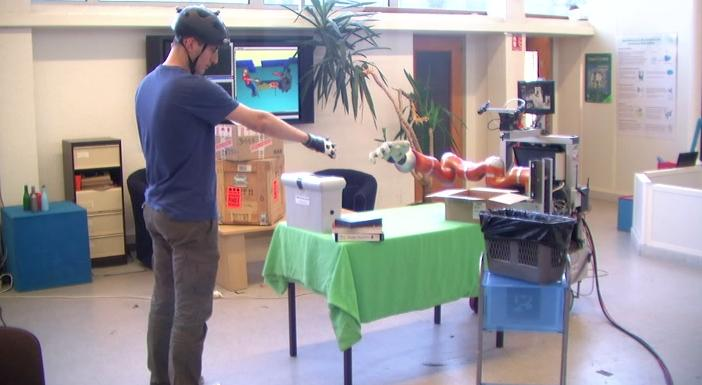
\includegraphics[width=0.9\linewidth]{images/dialogs/inTheBox2.jpg}
\caption{Jerry asks Jido for the content of the box by pointing at it.}
  \label{fig|pointing}
\end{figure}

In this situation, Jerry enters the
living room without knowing where Tom had placed the video tapes. So he first
asks Jido: ``What's in the box?''. Before the robot can answer the question it
has to figure out which box Jerry is talking about. Similar to the previous
situation, there are two available boxes: 

\begin{center}
\begin{tabular}{l}
\stmt{?obj type box}\\
\hspace{0.7cm}$\Rightarrow$ {\tt ?obj = [cardBoardBox, toolbox]}
\end{tabular}
\end{center}

However both are visible and the cognitive ambiguity resolution cannot be
applied. The only option is to ask Jerry which box he is referring to: ``Which
box, the toolbox or the cardboard box?'' Jerry could now simply answer the
question. Instead, he decides to point at it while indicating: ``This box''
(Figure~\ref{fig|pointing}). The robot's perception identifies the {\tt
cardBoardBox} as being pointed at and looked at by the human and updates the
ontology with this new information using a rule available in the commonsense
ontology ({\tt \textbf{pointsAt}(?ag, ?obj) $\land$ \textbf{looksAt}(?ag, ?obj) $\to$
\textbf{focusesOn}(?ag, ?obj)}) The \textsc{Dialogs} module is then able to merge both
sources of information, verbal (``this'') and gestural to distinguish the box
Jerry refers to.

\begin{center}
\begin{tabular}{l}
\stmt{Jerry pointsAt carboardBox}\\
\stmt{Jerry looksAt carboardBox}\\
$\to$ \stmt{Jerry focusesAt carboardBox}\\
\hspace{0.7cm}$\Rightarrow$ {\tt ?obj = [cardBoardBox]}
\end{tabular}
\end{center}

Finally, the \textsc{Dialogs} queries the ontology about the content of the box
and the question can be answered: ``Jido-E''. Note that the object's label is
used instead of its ID. This way we enhance interaction using familiar names
given by the users.

\begin{center}
\begin{tabular}{l}
\stmt{?obj isIn cardBoardBox}\\
\hspace{0.7cm}$\Rightarrow$ \concept{?obj = videoTape2}\\
\end{tabular}
\end{center}

At this point Jerry wants to know where the other tape is, and that is exactly
what he asks Jido: ``And where is the other tape?''. In this occasion, the
\textsc{Dialogs} module is able to interpret that Jerry is not referring to the
video which they were just talking about, but to the other one:

\begin{center}
\begin{tabular}{l}
\stmt{?obj type VideoTape}\\
\stmt{?obj differentFrom videoTape2}\\
\hspace{0.7cm}$\Rightarrow$ \concept{?obj = [videoTape1]}
\end{tabular}
\end{center}

Since there is only one possible ``other'' video (there are only two videos in
the scene), it can directly answer Jerry: ``The other tape is on the table and
next to the toolbox.''

\begin{center}
\begin{tabular}{l}
\stmt{videoTape1 isOn table}\\
\stmt{videoTape1 isNextTo toolbox}
\end{tabular}
\end{center}


\subsubsection{Second Interaction Experiment: ``Aperitif Time''}
\label{sect|expe2}

A similar experiment has been conducted in the appartment environment
(figure~\ref{fig|livingroom}) of the LAAS-CNRS with the PR2 robot.

\begin{figure}
    \centering
    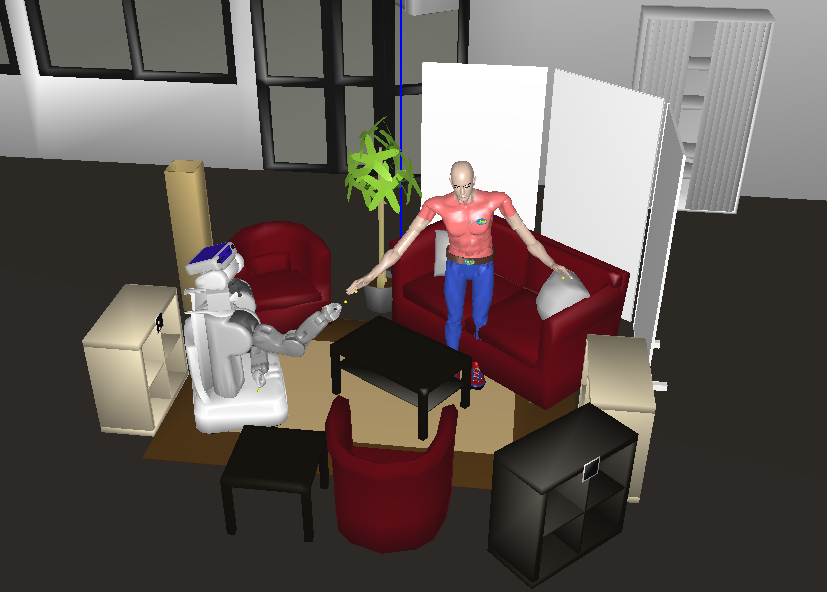
\includegraphics[width=0.7\columnwidth]{experiments/adream-livingroom.png}

    \caption{The ``Living room'' setup, as represented by the robot during the
    experiment.}

    \label{fig|livingroom}
\end{figure}

This second experiment is focused on verbal interaction, and the perception is
limited to the human tracking with a deported ASUS XTion (similar to the
Kinect) sensor. Contrary to the first experiment, objects in the environment
are not detected. Their positions are predefined. Pick\&Place manipulation
tasks are not planned either, and the robot gestures are predefined as well.

Dialogue with the robot goes through a custom Android application running on a
touchpad held by the human. This application relies on the Google Speech API
for text-to-speech recognition, and communicates exchange messages with the
robot via the XMPP/Jabber protocol.


\begin{figure}
    \centering
    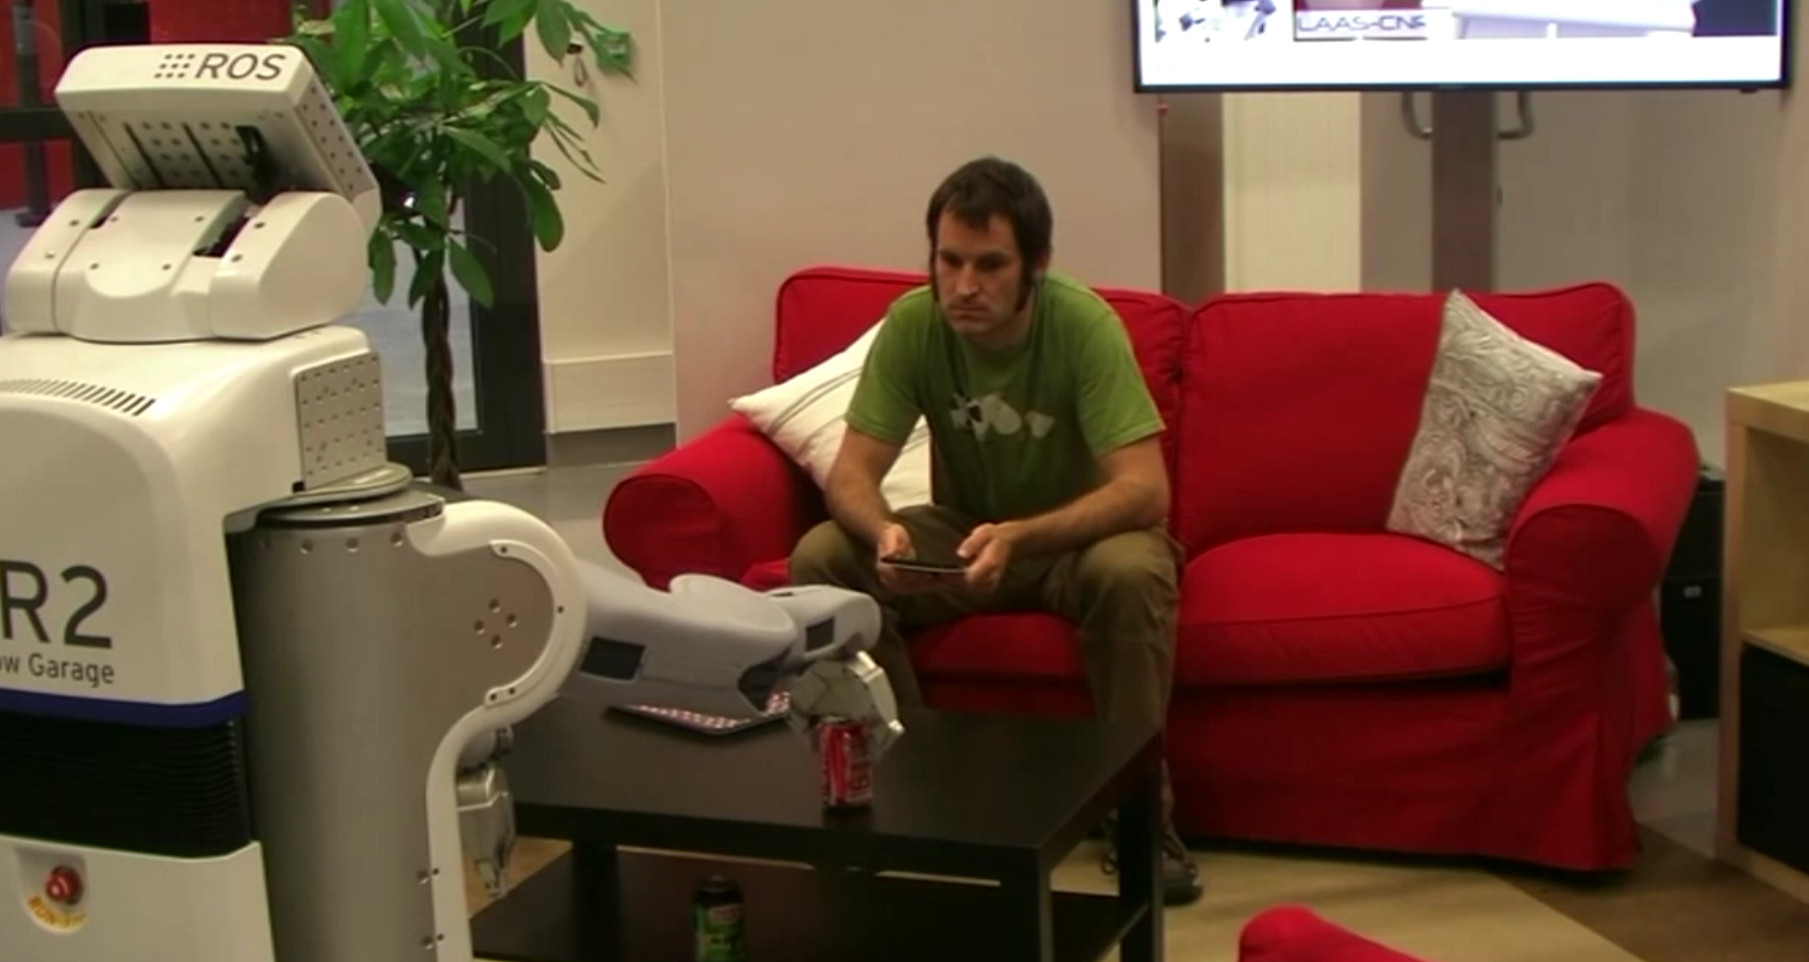
\includegraphics[width=0.9\columnwidth]{experiments/aperitiftime.jpg}
    \caption{This experiment led to a video that can be viewed online:
\url{http://www.youtube.com/watch?v=pLz8ifvtoeQ}.}
    \label{fig|aperitif-video}
\end{figure}

The experiment consists in manipulation of drinks (soda cans, wine minibottles)
by verbal commands that take into account the human perspective, and may
require discrimination (for instance, ``Give me the juice'' can refer either to
the orange juice or to the apple juice).

The reasoning and decisional principles are similar to the previous experiment,
and are not detailed here. This experiment can be considered as a more mature
version of the first one: more objects are involved, speech understanding is
vastly improved, the decisional layer is more developed (the {\tt pyRobots}
environment, briefly presented at section~\ref{sect|pyrobots}, is used to react
to incoming orders), the robot acts (pick \& place, tracking of the human with
the head, etc.).

\paragraph{Evaluation} The results of these two first experiments is however
not fully satisfactory.

\begin{itemize}

    \item the complexity of the system makes it error prone. Besides, lack of
        sufficient decoupling between the higher-level components can lead to
        long restart procedures. In particular, the ORO knowledge base also has
        stability issues (reasoner crashes), that greatly vary with the
        ontology content, in ways that are difficult to predict.

    \item in the first experiment, the tag-based tracking of object is fragile
        (sensible to partial occlusions, lighting conditions, etc.), while in
        the second experiment, the absence of tracking of objects (due in part
        to the size of cans, too small to stick a tag, in part to the desire to
        avoid altogether perception issues in the system, and in part to the
        location of objects, sometimes only partially visible, like the can on
        the bottom of the picture~\ref{fig|aperitif-video}) leads obviously to
        poor robustness of manipulation tasks.

    \item ...
\end{itemize}

It must be also noted that the second experiment has been originally designed
as a user-study: a naive, non-expert user was given a list of drinks to ask the
robot to prepare for the aperitif. The idea was to compare the time required
for the task achievement with several conditions, including use or not of
perspective taking. We gave up with this project because of the lack of good
enough resillience of the dialogue system to non-expert inputs. For instance
ill-formed English sentences or elliptic sentences are not dealt correctly
with. A pre-study that was meant to gather example of verbal inputs and
involving about fifty users has been however conducted. It provides a valuable
database to exercice and further develop the dialogue management system.

\subsubsection{Third Interaction Experiment: ``Cleaning the Table''}
\label{sect|expe3}

The third experiment involved a more complex decisional layer where the ORO
server was used in conjunction with the HATP symbolic task planner and the
SHARY execution controller (the complete software architecture we deployed for
this experiment is pictured on figure~\ref{fig|archi},
page~\pageref{fig|archi}).

In this scenario (figure~\ref{fig|cleantable-video}), a human and a robot
cooperate to remove objects from a table. The robot produces symbolic plans for
both itself and the human (\cite{Alami2011}, see also section~\ref{sect|hatp})
that allow the robot to (verbally) share the task with the human (like ``I take
the green box and I put it in the trashbin, you take the black video tape and
you throw it in the trashbin''). Plans are created based on perceived
visibility and reachability of the objects, and the robot also monitors the
human activities to track the advancement of the whole plan (this last aspect
is presented in~\cite{Warnier2012}).

\begin{figure}
    \centering
    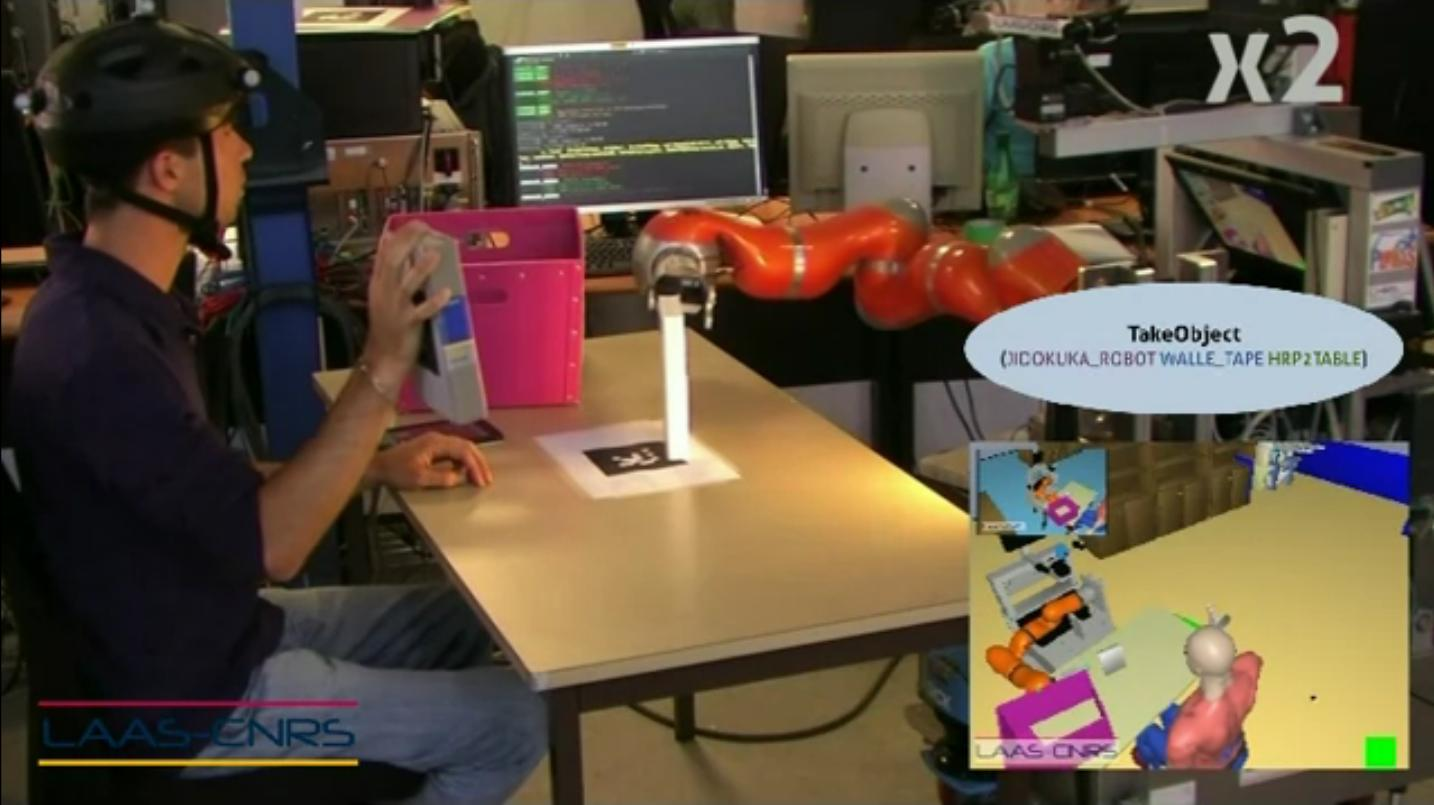
\includegraphics[width=0.7\columnwidth]{experiments/cleantable.jpg}
    \caption{}
    \label{fig|cleantable-video}
\end{figure}


Figure~\ref{fig|cleantable-timeline} presents a excerpt of the whole task and
shows how the different components produce and use symbolic knowledge (note
that the plan is actually computed {\it a priori}. It appears nevertheless on
this diagram for better readability).

\begin{figure}
    \centering
    \includegraphics[width=\columnwidth]{experiments/manip_run.pdf}

    \caption{This diagram shows a simplified version of the ``Clean the Table'' scenario timeline.}

    \label{fig|cleantable-timeline}
\end{figure}


This experiment also led to a video that can be viewed online:
\url{http://www.youtube.com/watch?v=IODx50uV_k4}.


\subsection{The Roboscopie performance}
\label{sect|roboscopie}

The last experimental setup we have been working on is less usual, since it is
a theatre performance, involving one human actor and the PR2 robot.

Theatre with robotic actors is an emerging field, with a few previous published
results~\cite{Breazeal2003, Lin2009, Mavridis2009}.

On the 14th of October 2011, we performed for a general public audience (over
300 persons) a 18 min long live theatre play, acted by professional actor
Xavier Brossard and the LAAS/CNRS PR2 robot. The play was created and directed
by Nicolas Darrot, a mixed-media artist from Paris.

The PR2 was programmed in a 2-months course, re-using several software
components presented in this thesis, including the 3D environment for situation
assessment SPARK, the knowledge base ORO and the natural-language
processor {\sc Dialogs}.

This section presents the storyline of the play, gives details on the technical
side of the project, and underlines some of the significant outcome from the
human-robot interaction perspective.

Both a short teaser and the full-length version of the performance are
available from a dedicated website, \url{www.laas.fr/roboscopie}.

\begin{figure}
    \centering
    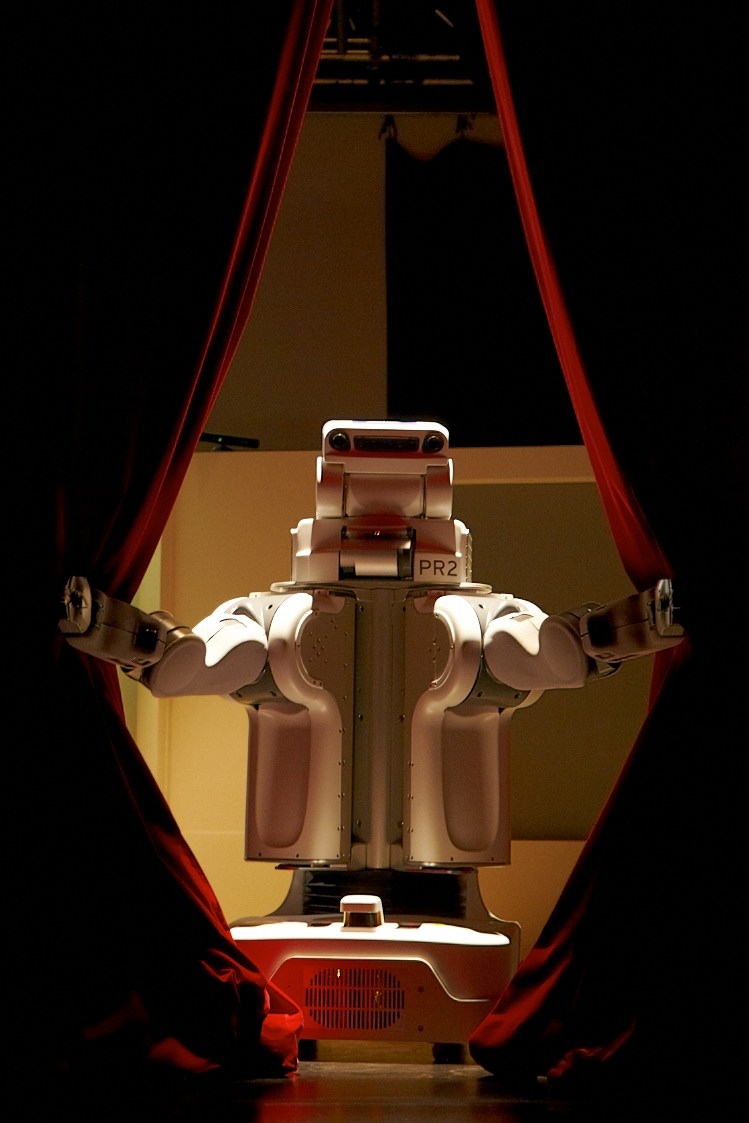
\includegraphics[width=0.5\columnwidth]{experiments/roboscopie.jpg}
    \caption{The PR2 robot at the beginning of the performance.}
    \label{fig|pr2-opens-curtains}
\end{figure}


\subsubsection{Storyline}

The play discusses how humans and robots can find a common ground for understanding
each other, by living in a kind of frontier world, where real objects are replaced 
by abstract, disembodied counterparts.

Xavier and PR2 share a white, almost empty, stage. To get the robot to see his
world, Xavier must keep being recognized by the human tracking module that lies
on the wall, and must stick everywhere 2D barcodes, instead of real
objects. The robot can read and identify these barcodes, and while the stage
gets covered by the tags, the robot constructs for itself a 3D world with the
right-looking objects: a phone, a lamp, a hanger...

While Xavier is drawing by hand more and more of these 2D tags, the robot tries
to offer its help. It brings first a bottle of water, then a fan... which blows
away all Xavier's code. Angry, Xavier leaves, and PR2 remains alone.

The night comes, and the robot decides to explore the stage, scattered with
those barcodes on the ground. On the next morning, Xavier discovers that the
robot's 3D model is a mess, full of random objects: an elephant, a boat, a
van... Xavier resets the robot model and starts to tidy up the place. The robot
decides to help with a trash bin, but suddenly gives up and a new program
starts: a home-training session. Xavier starts the exercises, but as the
program goes along, the robot looks more and more menacing, up to the point
that Xavier shouts "Stop!".

Xavier eventually shows one after the other the objects to the robot,
explaining they are all fake, and like the robot, we realize that everything
was just an experiment.

\subsubsection{Technical overview}

The PR2 robot was running softwares developed at the LAAS/CNRS. While the
performance tries to picture some of the challenges in the human-robot
interaction field, including the needed autonomy of a robot working with
humans, the robot was partially pre-programmed for this theatre performance.

Most of the behaviours were coded in Python, relying both on the PR2 ROS
middleware and on {\sc GenoM}, the LAAS own middleware.

\begin{figure}
    \centering
    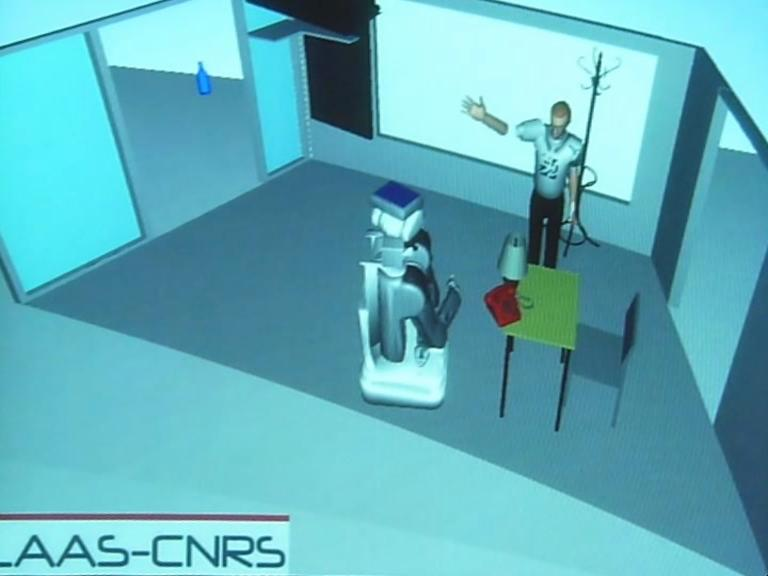
\includegraphics[width=0.8\columnwidth]{experiments/roboscopie-spark.jpg}
    \caption{The robot build a coherent 3D model of its environment through the
    SPARK module}
    \label{fig|spark}
\end{figure}

\paragraph{What was pre-programmed?}

General behaviour: While the real perception routines were running
(see next section), the robot did not have any mean of synchronization with the
human during the play: each sequence was manually started by one of the
engineers.

Places on the stage were hard-coded: for instance, the position of the table
was known to the robot from the beginning, so was the position of the entrance
door, etc.

Postures and manipulation tasks: Manipulation tasks (like grasping
the fan or the paper bin) were much simplified: the robot would simply open its
gripper, and wait for \emph{something} to be detected in its hand. It would
then simply close the gripper. Likewise, the robot special postures to enter or
leave the stage with an object in hand (required to avoid collision with the
door) were all pre-defined.

Speech Understanding: At the end of the play, when Xavier talks to
the robot (\emph{Stop!}, \emph{Look at this phone!}, \emph{Everything is fake},
etc.), sentences were manually typed in the system. We could have used speech
recognition as we do in the laboratory, but converting speech to its textual
version is relatively slow and error prone. So we decided to avoid it on the
stage.

While what Xavier said was actually processed by the robot (see next section),
the actions that followed (like looking at the phone, turning the head back to
the audience,...) were manually triggered.

\paragraph{What was autonomously managed by the robot?}

Navigation: All navigation tasks were computed \emph{live} by
PR2, using the ROS navigation stack. The main script just tells the robot to go
from the engineer desk to the center of the stage for instance. The robot would
then find a path that avoid obstacle.  

Modeling of the environment: The 3D world that is displayed above
the stage during the show (Fig.~\ref{fig|spark}) is a live capture of the
Move3D and SPARK softwares. These softwares are used daily on the robot to
compute trajectories, symbolic locations, visibility and reachability of
objects, etc.

However, during the performance, we deactivated the computation of symbolic
facts (like {\tt xavier looksAt jacket}, {\tt RED\_PHONE isOn table},...) which
is not reliable enough to be used on the stage.

The 2D barcodes are actually a key perception mechanism for our PR2. They are
well identified {\sc ARToolkit} tags used to identify and localize (both for the
position and the orientation) objects surrounding the robot.

Besides, the robot was able to track the human whole-body posture with a
Microsoft Kinect sensor and the {\sc OpenNI} human tracker. In several
occasion, the robot automatically tracks the human head or the human hands with
this system.

Speech Understanding: At the end, Xavier talks to the robot. The
textual version of what he said was fed to the system \emph{as it}. Natural
language understanding is done by the {\tt Dialogs}
module~\cite{Lemaignan2011a} and used extensively the {\tt oro-server} knowledge
database to make sense of the word in the current context. The result of the
language processing was then added back to the knowledge base and automatically
displayed by the {\tt oro-view} OpenGL ontologies viewer.

Hence, the sentence \emph{``look at this phone''} get translated into symbolic
facts: {\tt [human desires action1, action1 type Look, action1 receivedBy
RED\_PHONE]}. The robot is able to know that <this phone> is indeed the {\tt
RED\_PHONE} by taking into account what the human focuses on.

Since the computation of symbolic facts was deactivated, we had to manually add
several symbolic facts in a so-called scenario-specific ontology.

\subsubsection{Significance for HRI}

A first noteworthy achievement of this project from the human-robot
interaction point of view is the use and display of the set of research tools
developed at LAAS in front of a general audience: while the show had been
precisely scripted and rehearsed, the robot was running the same software
components we use on a daily basis in the laboratory.

By building the performance storyline on the current, actual state of robotic
research,  the play also put light on three key questions of today's
human-robot interaction: how the human and the robot can understand each others
(the robot tries to help but remains intrusive)? how to share and coexist in a
common living space? how roles build up between the human and the robot (who
dominates)?

